\documentclass[11pt,a4paper,openany]{book}


\usepackage{amsmath}

\usepackage{graphicx}

\usepackage{hyperref}

\usepackage[utf8]{inputenc}



\begin{document}
\newpage
\thispagestyle{empty}

\baselineskip 2em

%\vspace*{1cm}

\centerline{
\includegraphics[width=0.6\textwidth]{images/UOC-logo}}
\begin{center}
\textsc{Universitat Oberta de Catalunya (UOC) \\
 Máster Universitario en Ciencia de Datos (\textit{Data Science})\\}

%\centerline {\pic{UOC}{4cm}}

\vspace*{1.5cm}

\textsc{\Large TRABAJO FINAL DE MÁSTER}

\vspace*{0.5cm}

\textsc{\large Área: YYY}


%\textbf{\Huge VirtualTechLab Model: }

\vspace*{2.0cm}

\title{\Large Artificial MRI brain images creation with Variational Autoencoders}

\vspace{2.5cm}
\baselineskip 1em

\baselineskip 2em
-----------------------------------------------------------------------------\\
Autor:      Miguel Tablado\\
Tutor:      Baris Kanber\\
Profesor:   Nombre del profesor responsable del área de TF\\
-----------------------------------------------------------------------------\\
\vspace*{1.5cm}
Barcelona, \today

\author{Miguel Tablado}

\end{center}
\hfill


\tableofcontents

%%%%%%%%%%%%%
%%% FICHA %%%
%%%%%%%%%%%%%
\chapter*{FICHA DEL TRABAJO FINAL}
\begin{table}[ht]
	\centering{}
	\renewcommand{\arraystretch}{2}
	\begin{tabular}{r | l}
		\hline
		Título del trabajo: & Artificial MRI brain images creation with Variational Autoencoders\\
		\hline
        Nombre del autor: & Miguel Tablado León\\
		\hline
        Nombre del Tutor/a de TF: & Baris Kanber\\
		\hline
        Nombre del/de la PRA: & Baris Kanber\\
		\hline
        Fecha de entrega: & 02/2023\\
		\hline
        Titulación o programa: & Máster en Ciencia de Datos\\
		\hline
        Área del Trabajo Final: & Area Medicina (TFM-Med)\\
		\hline
        Language: & English\\
		\hline
        Keywords & Deep Learning, Brain MRI, Variational Autoencoder\\
		\hline
	\end{tabular}
\end{table}

\chapter*{\centering Abstract}
\addcontentsline{toc}{chapter}{Abstract}
\begin{quote}
    {Artificial Intelligence is set to be key technology at medicine projects in where models will help doctors at diagnostics with image processing. Magnetic Resonance Images allow doctors to scan brains and create a images that can be used for training models. However, it is too expensive and slow to be able to create large dataset required for models to work at highest accuracy and this project aims to create artificial brain MR images that would enlarge the base dataset combining with real images.
    
    A potential use case in where AI-generated images could be used are anomaly detection by comparing an input image with healthy images to detect if it presents any anomaly to be analyzed by a doctor.
    
    During this project Variational Autoencoders will be used in order to create new images where different existing network architectures will be analyzed before working on the performance tuning with the one which brings better results at initial analysis.
    
    The duration of the project implementation will start on October 24th and will end up by December 25th with one Data Scientist working on the project with a budget of 300 hours that will be distributed during that frame and that will require GPU computation for processing the different training and testing networks.
    
    This project aims to be a Proof of Concept and the resulting images will be visually analyzed and compared to real images to check if the network is able to generate images that could be used as valid images.}
\end{quote}

\chapter{Introduction}

\section{Context and project justification}

Artificial Intelligence has arrived to change the world in almost (if not all) any field. Today, we are surrounded by (and we are using many) AI products like smartphones’ face recognition capabilities, home cleaning robots or cars with autopilot options.

From the different AI fields, computer vision is maybe the most popular one and the one which is usually used for explaining AI capabilities to general public. Identifying a cat in a picture could perfectly be the example used in every AI presentation to welcome people to AI.

Image processing is intuitively matched with medical diagnosis by anyone having or not any expertise on the field. Every single citizen will have heard of magnetic resonance imaging, and anyone easily transposes ‘cat detection’ to ‘anomaly detection’, being the anomaly a tumor or anything else.

There are different techniques to scan people and create images for clinical diagnosis like X-Ray or Magnetic Resonance Imaging. In this project, we will work with Magnetic Resonance Images (MRI) which are images created by a machine with a large bore that scans people lying inside it. The MR technique is non-invasive, it produces no radiation, and is used to scan almost any part of the body from which this thesis will focus on brain images.

Combining AI diagnosis capabilities on image processing and MRI images, you can think of helping doctors to identify the presence of anomalies or looking for concrete diagnosis for a specific disease.

Obviously, these projects are not easy at all and they face a lot of challenges. One of the first challenges that such AI project faces is the difficulty to obtain a large set of brain images that are needed to train an accurate AI model. Scanning people is too costly and requires a lot of time and the challenge of having a large dataset gets harder once we understand that brain images may differ depending on age or gender.

Today, there is a clear limitation on how to reproduce or obtain healthy brain images for AI-based diagnosis projects while the appearance of new AI techniques known as Autoencoders and Variational Autoencoders introduces a new area of investigation to mitigate the gap.

This project aims to be a proof of concept to create AI-created images with new variational autoencoders that would serve to augment any existing MRI dataset and that will help to improve the accuracy of brain anomaly detection projects, including those which could be used for overall anomaly detection to others more specific which would help on concrete disease diagnosis.

When submitted, Dr Baris Kanber's thesis proposal was intended to use Autoencoders for MRI reconstruction of images. However, some alternatives were propopsed by him during the first presentation meeting to go beyond that. Dr Baris Kanber suggested to use Variational Autoencoders first, then varying the project objective to create new artificial images instead of recreating them by using the latent space probability distributions. Both proposals were taken with even when more research and experiments would be needed due to the lack of previous projects using this technique.

Variational Autoencoders are seen as an evolution of Autoencoders which store discrete values of each attribute in the latent space while VAEs uses probability distributions. This will be described deeper later in this document. 

Personal motivation comes from various angles:

\begin{itemize}
    \item One is to prove myself that I can work with new AI architectures demonstrating that I have acquired the knowledge needed (deep enough) to be productive and to be able to innovate in the health sector.
    \item Deep Learning has been the subject which I enjoyed the most, hence continuing with Autoencoders seems natural to me as the next step on AI adoption
    \item At no doubts, if I can contribute to help on brain issue detection or diagnosis, I will feel my life been completely fulfilled
\end{itemize}
\section{Aim of the project}

The aim of this project is to serve as a Proof of Concept on how MRI brain images can be artificially generated with Variational Autoencoders which ultimately would serve to enhance existing or new datasets to improve model accuracy by having larger samples of data.

Foreseen projects objectives are:

\begin{itemize}
    \item Obtain basic knowledge about MRI images and the NIFTI file format
    \item Obtain and visualise 2-D images from 3-D images in the dataset
    \item Select what range of slices (2-D images) from brain to be created
    \item Test different existing networks and choose the one to be used
    \item Tune network parameters
    \item Compare generated brain images against real ones, qualitatively
\end{itemize}
\section{Project Plan}

\subsection{Resources}

\begin{enumerate}
    \item 1 Data Scientist: Miguel Tablado will be playing this role and will dedicate 300h
    \item 1 Coach/Tutor: Baris Kanber will be assisting Miguel Tablado during the project
    \item MRI images and demographic information from IXI Dataset
    \item GPU resources are needed to train and test the network
\end{enumerate}

\subsection{High Level Plan}

The plan will be executed in 3 different phases with the listed tasks:
\begin{enumerate}
    \item Phase 1: Analysis
    \begin{enumerate}
        \item Gain knowledge on MRI and NIFTI protocol
        \item Describe images and dataset
        \item Extract 2D images
        \item Pre-processing images
    \end{enumerate}
    \item Phase 2: MR Images creation
    \begin{enumerate}
        \item Test different Network architectures
        \item Tune-up architectural network
    \end{enumerate}
    \item Phase 3: Project documentation
    \begin{enumerate}
        \item Write conclusions
        \item Create project documentation
        \item Create project presentation
    \end{enumerate}
\end{enumerate}

\begin{figure}[ht]
    \hspace*{-1.2in}
    \centering
    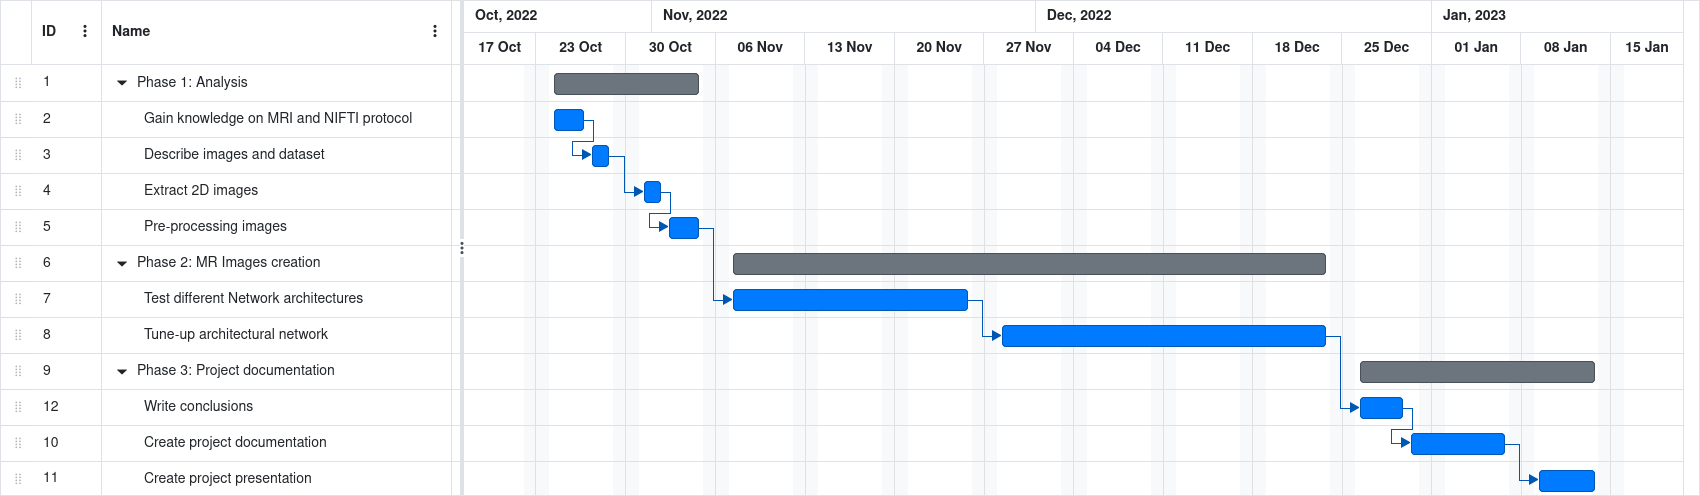
\includegraphics[width = 20cm, height = 6cm]{images/project-plan.png}
    \caption[]{Project Plan. source: https://www.onlinegantt.com}
    \label{fig:project-plan}
\end{figure}



\end{document}
